\section{Analysis of Internal Path Length}
\subsection{Theoretical Study}
Let \( T \) be a BST of size \( n \) with root \( r \). We define the \textit{Internal Path Length} of \( T \) as the sum of all distances between every node of the tree and the root. More formally:  
\[
\text{IPL}(T) = \sum\limits_{v \in V(T)} d(r,v).
\]
This metric should not be surprising, as we can estimate the distance between the root and every node by averaging the IPL of such a tree. Before establishing this relationship, let us first derive a recurrence for the IPL of a tree, solve this recurrence, and later analyze the obtained relation.

Under the assumption of having a random BST, given \( n \) keys, we consider every permutation among the \( n! \) possible ones to be equally likely. Therefore, the sizes of the subtrees \( T_l \) and \( T_r \) will be completely random, provided that their combined sizes sum to \( n - 1 \). Consequently, in our recurrence, we must consider every possible size distribution of the subtrees as equally likely.

Moreover, given the IPL of \( T_l \) and \( T_r \), since we introduce a new root at the top of the tree, every node will need to traverse one additional edge to reach the new root. This results in adding \( 1 \) to the previous distances with respect to their original root. As a consequence, we must add the number of edges in the tree to the sum of the previous IPLs of both subtrees.

Hence, creating the following recurrence:

\begin{align*}
    IPL_n &= n - 1 + \frac{1}{n}\sum\limits_{k = 0}^{n-1} IPL_k + IPL_{n-1-k} \\
        &= n - 1 + \frac{1}{n}\sum\limits_{k = 0}^{n-1} 2 \cdot IPL_k \\
        &= n - 1 + \frac{2}{n}\sum\limits_{k = 0}^{n-1} IPL_k \\
\end{align*}

We can, again, use the continuous master theorem in order to solve this recurrence. Again we need to determinate the following values:

\begin{itemize}
    \item Determine the values of \( a \) and \( b \): Since \( t_n = \Theta(n) \), it is straightforward to see that $a = 1$ and $b = 0$.
    \item Provide a shape function for the weights \( w_{n,j} \): We use the following trick to determine the shape function:

    \[
    w(z) = \lim\limits_{n\to\infty} n \cdot w_{n,z\cdot n} = n \cdot \frac{2}{n} = 2.
    \]

    \item Determine the value of 

    \[
    \mathcal{H} = 1 - \int\limits_{0}^{1} w(z) z^a dz.
    \]

    Substituting the values, we obtain:

    \[
    \mathcal{H} = 1 - \int\limits_{0}^{1} 2z dz = 1 - (1 - 0) = 0
    \]

    \item Since \( \mathcal{H} < 0 \) we are in the case

    \[
    \mathcal{H'} = -(b+1) \int\limits_{0}^{1} w(z) z^a \ln z \, dz.
    \]

    Substituting the known values,

    \[
    \mathcal{H'} = -1 \int\limits_{0}^{1} 2z \ln z \, dz.
    \]

    This integral can be solved using integration by parts. For the purpose of applying the theorem, we skip the detailed calculation, giving the result:

    \[
    \mathcal{H'} = - (x^2 \ln x - \frac{x^2}{2})\Big|_0^1 = \frac{1}{2}.
    \]

\end{itemize}

Since \( \mathcal{H} = 0 \) and \( \mathcal{H'} \neq 0 \), we use the result

\[
F_n = \frac{t_n}{\mathcal{H'}} \ln n + o(t_n \log n).
\]

Substituting the values, we obtain

\[
I_n = 2(n-1) \ln n + o(n \log n) = 2n \ln n + o(n \log n)
\]

Thus, the expected internal path length in a BST is bounded by \( O(n \log n) \). Such recurrence can be used to solve the expected cost of doing an insertion in a BST as we can express that cost as: $I_n = 1 + \frac{IPL_n}{n}$ (as we can have an estimation of $I_n$ by averaging the internal path length over the size of the tree in order to get an estimation of the average distance between the root and a node) which would give a result of $O(\log n)$ which was the expected bound we obtained in the previous section.

\subsection{Experimental Study}
Once we have theoretical results on the expected internal path length in a random BST, we can provide experimental results to assess how closely they match the theoretical predictions. For this, we will conduct the following experiment:

\begin{enumerate}
    \item We create a random BST of size \( n \) by generating \( n \) random keys in the interval \( [0,1] \).
    \item We calculate the internal path length of the random BST by doing a Breadth-first search algorithm
    \item We repeat all previous steps with 20 different seeds and compute the final average.
    \item We repeat the entire experiment for different values of \( n \).
\end{enumerate}

Again, I conducted the experiment with the same value of $n$ and same values of \textit{seeds} as before. Figure \ref{fig:plotBoundIPL} provides, as before, a plot with the expected values we should obtain following the continuous master theorem result and the experimental result. This time we do not see a similar behavior between the two curves as we saw before: It seems that the theoretical bound increase faster than the experimental result, not at the same time as before.

\begin{figure}
    \centering
    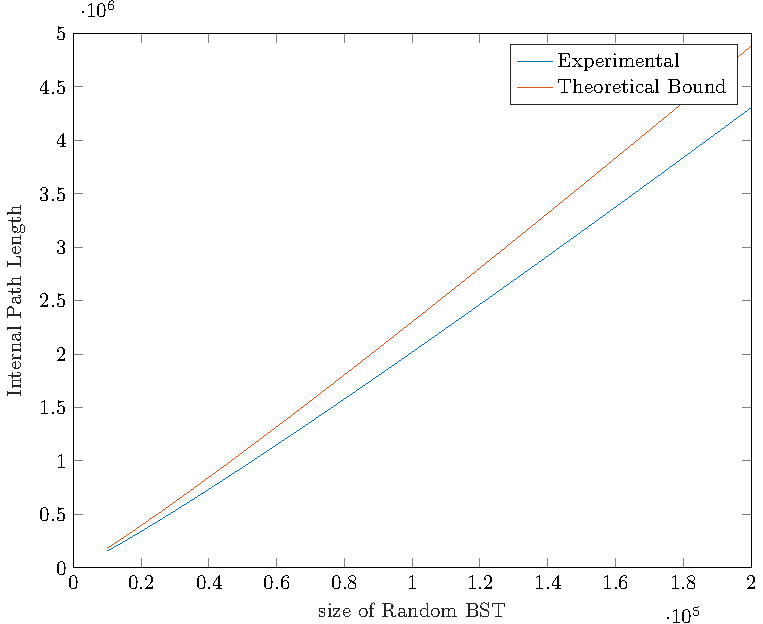
\includegraphics[scale=0.65]{plotIPL.pdf}
    \caption{Plot average IPL respect the theoretical bound}
    \label{fig:plotBoundIPL}
\end{figure}

We know that there is a factor \( o(n \log n) \) (in fact, with a more detailed solution of the recurrence, see Appendix CITAR, we know that this $o(n \log n)$ is $O(n)$) that must be taken into account in our study. As a result, even with a high number of nodes in a random BST, this theoretical bound may still be influenced by the \( o(n \log n) \) factor until we reach a significantly larger number of nodes. To analyze this effect, we provide Figure \ref{fig:plotBoundCtIPL}, where we divide the experimental data by \( n \log n \) to observe when this \( o(n \log n) \) factor stabilizes. As seen in the figure, even for large input sizes (over 200,000 nodes), this factor still plays a significant role in our analysis.

\begin{figure}[ht]
    \centering
    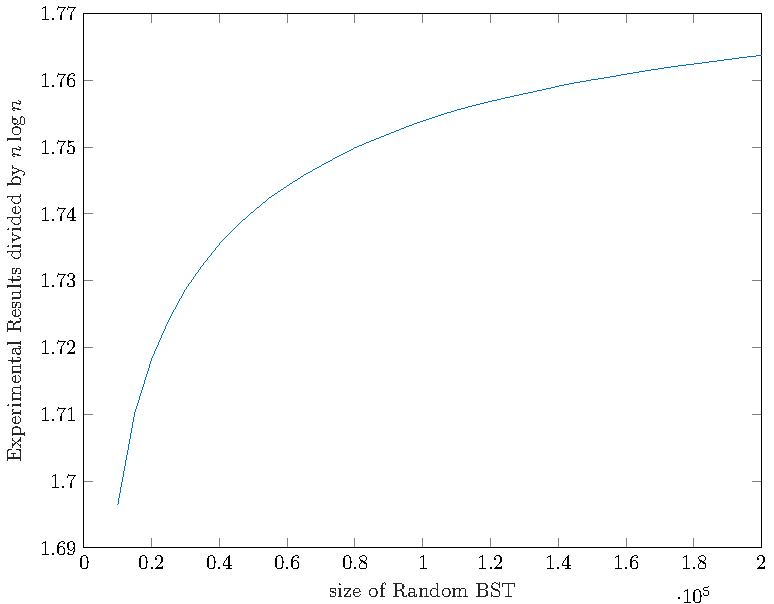
\includegraphics[scale=0.65]{plotCtIPL.pdf}
    \caption{Plot experimental result divided by $n \log n$}
    \label{fig:plotBoundCtIPL}
\end{figure}
